% Dieser Text ist urheberrechtlich geschützt
% Er stellt einen Auszug eines von mir erstellten Referates dar
% und darf nicht gewerblich genutzt werden
% die private bzw. Studiums bezogen Nutzung ist frei
% Nov. 2007
% Autor: Sascha Frank 
% Universität Freiburg 
% www.informatik.uni-freiburg.de/~frank/
\documentclass[handout]{beamer}
\setbeamertemplate{navigation symbols}{}
\usepackage[utf8x]{inputenc}
\usepackage[T1]{fontenc}
\usepackage{pgfplots}
\usepackage{siunitx}
\usepackage{graphicx}


\newlength\figureheight
\newlength\figurewidth


\usetheme{Montpellier}
%\usecolortheme{beaver}
%\usepackage{ngerman}
%\beamersetuncovermixins{\opaqueness<1>{25}}{\opaqueness<2->{15}}

%\setbeamercovered{invisible}
\begin{document}
\title{Digit recognition and adversarial examples}
%\subtitle{Analysis of Data from Monkey Cerebral Cortex}  
\author{Jan-Hendrik Plank, Jonas Dehning \& Philipp Höhne}
\date{\today} 
%\titlegraphic{\includegraphics[width=\textwidth,height=.5\textheight]{someimage}}


\begin{frame}
\titlepage
\end{frame} 

%\begin{frame}
%\frametitle{Table of Contents}\tableofcontents
%\end{frame} 

%\section{Digit recognition}

\begin{frame}
\frametitle{Digit recognition} 
\begin{figure}
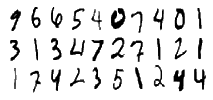
\includegraphics[width=0.5\linewidth]{./front_page.png}
\end{figure}
\begin{itemize}
\item Method: deep convolution network
\item MNIST-Dataset
\item 28000 images: 28px $\times$ 28px
\end{itemize}
\end{frame} 
%slide numbering
%videa scrambling, temporal receptor fields larger uri hasson
%summary slide
%changes of task

\begin{frame}
\frametitle{Adversarial examples}
\begin{itemize}
\item Small pertubations $\rightarrow$ false classification
\end{itemize}
\begin{figure}
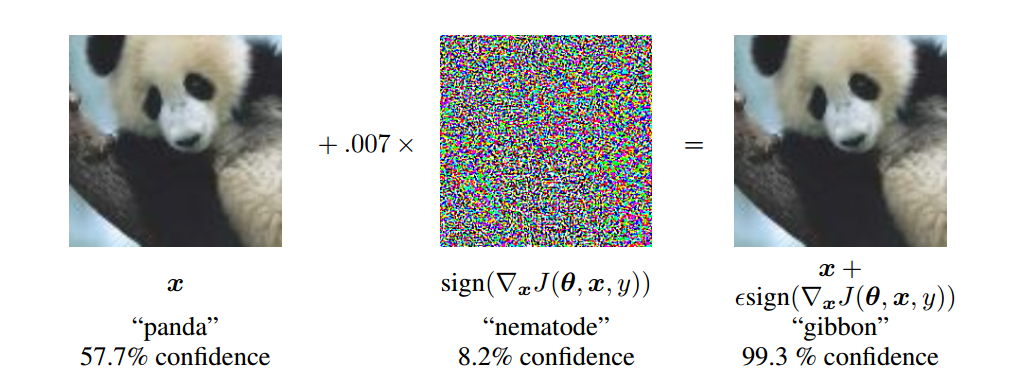
\includegraphics[width=0.9\linewidth]{./PandaGibbon}
\end{figure}
\begin{itemize}
\item From Goodfellow et al. 2015
\end{itemize}
\end{frame}

\begin{frame}
\frametitle{Further ideas}
\begin{itemize}
\item improve network by training with the perturbed images
\begin{itemize}
\item improved kaggle score?
\end{itemize}
\item compare different datasets
\item compare robustness of different networks
\end{itemize}
\end{frame}














\end{document}